\chapter{Analysis Framework}
\label{ch:framework}

This section defines our analytical framework for evaluating how geometry-model-based feature distillation affects MLLM performance on VLN. Specifically, we systematically investigate the effects of teacher model architecture, information flow directionality, and the temporal stride of navigation history on distillation efficacy and navigation performance.

\section{MLLM Baseline}
\label{sec:mllm_baseline}

In VLN, an agent predicts the next action $a_{t+1}$ conditioned on a natural language instruction $I$ and the sequence of RGB observations up to timestep $t$, $\mathcal{O}_t = \{x_1, \dots, x_t\}$. The action space consists of \texttt{MOVE\_FORWARD}, \texttt{TURN\_LEFT}, \texttt{TURN\_RIGHT}, and \texttt{STOP}, and the agent's policy is formulated as:

\[
a_{t+1} \sim \pi(\cdot \mid \mathcal{O}_t, I)
\]

Our baseline is an MLLM adapted to VLN via supervised fine-tuning (SFT). The agent operates in a multi-turn dialogue format, predicting 4 consecutive actions per turn. After executing every 4 actions, a new observation image is appended to the dialogue; once 8 turns of predictions are completed, the context is reset and a new dialogue begins. Each dialogue is initialized with the natural language instruction $I$ and a navigation history consisting of the preceding 8 observation images sampled at 4-step intervals.

\section{Teacher Models}
\label{sec:teacher_models}

\textbf{VGGT~\cite{wang2025vggt}} is a feed-forward transformer that jointly predicts camera parameters, depth maps, pointmaps, and 3D point tracks from single or multiple RGB images in a forward pass. Each input image is tokenized into patches via DINOv2~\cite{oquab2024dinov2} and augmented with learnable camera and register tokens. The resulting sequence passes through an Alternating-Attention backbone that interleaves frame-wise self-attention with bidirectional global self-attention across all frames. A camera head then estimates camera intrinsics and extrinsics from the camera tokens, while a DPT head~\cite{ranftl2021vision} aggregates intermediate features from multiple backbone layers for dense predictions, including depth maps and viewpoint-invariant pointmaps.

\textbf{Pi3~\cite{wang2026permutation}} is a permutation-equivariant visual geometry model designed to eliminate the input-order sensitivity and inductive bias introduced by anchoring coordinates to a fixed reference view. Like VGGT, it tokenizes images using DINOv2, but removes order-dependent components and exchanges multi-view information across 36 layers of alternating view-wise and global self-attention initialized from VGGT weights. Rather than employing a DPT head that fuses multi-layer intermediate features, Pi3 applies a lightweight transformer decoder that independently processes final-layer backbone features per view, followed by MLP and pixel-shuffle output heads. This enables the prediction of scale-invariant local pointmaps in each frame's own coordinate system without a global reference frame, alongside affine-invariant camera poses supervised by relative poses.

\textbf{DepthAnything3 (DA3)~\cite{lin2025depth}} unifies monocular and any-view 3D geometry reconstruction using a single plain transformer and a depth-ray representation, avoiding specialized architectures and redundant multi-task targets. It adopts a pretrained vanilla DINOv2 backbone without structural modifications. Within the transformer backbone, early layers perform only within-view self-attention, whereas later layers alternate between cross-view self-attention (via token rearrangement) and within-view self-attention. For output decoding, a Dual-DPT head~\cite{ranftl2021vision} processes multi-layer backbone features through a shared reassembly module and separate fusion branches to jointly predict dense depth maps and per-pixel ray maps.

\textbf{CUT3R~\cite{wang2025continuous}} is a stateful recurrent 3D perception model that processes image sequences sequentially while continuously updating a persistent state. Each frame passes through a shared ViT~\cite{dosovitskiy2021an} encoder initialized with DUSt3R~\cite{wang2024dust3r} weights and a ViT-Base transformer decoder. At every timestep, the model simultaneously performs a state-update to integrate the current observation into the persistent state and a state-readout to inject past 3D context into the image tokens. From the post-decoder image and pose tokens, it predicts metric-scale pointmaps in both local and world frames via a DPT head~\cite{ranftl2021vision} and 6-DoF ego-motion via an MLP head. While CUT3R defaults to unidirectional online inference conditioned only on past and current observations, it also supports bidirectional global context through a revisiting mode, which accumulates and fixes the final state over a first pass before re-encoding the same sequence.

\section{Directionality of Information Flow}
\label{sec:directionality}

Most multi-view geometry models rely on bidirectional information exchange when encoding image sequences. By contrast, a student MLLM's causal attention permits only unidirectional information flow, potentially making it difficult for the student to predict teacher target features that encode future frame information. To investigate how teacher encoding directionality affects target feature quality and VLN performance, we construct controlled comparisons across two model families.

\textbf{VGGT Variants.} VGGT incorporates future frame context into current frame representations via bidirectional global attention. We compare it against two causal variants. First, causal VGGT retains the pretrained VGGT weights unchanged while applying a causal mask solely to the bidirectional global attention layers. Second, to control for potential representation degradation caused by the mismatch between bidirectional pretraining and inference-time causal masking, we evaluate StreamVGGT~\cite{zhuo2026streamvggt}, which is trained directly with temporal causal attention.

\textbf{CUT3R Variants.} CUT3R performs sequential inference via its recurrent architecture and can incorporate bidirectional global context through revisiting mode, which accumulates hidden states in a first unidirectional pass and re-encodes the sequence in a second pass. We compare bidirectional inference (with revisiting) against unidirectional inference (without revisiting) to assess the role of information flow directionality in recurrent teachers.

\section{Temporal Stride in Context}
\label{sec:temporal_stride}

Because multi-view geometry models infer 3D structure from cross-frame visual correspondences, they are sensitive to the temporal spacing between context frames. In our default configuration, the navigation history samples the preceding 8 images at 4-step intervals. To examine the interplay between long-horizon context acquisition and 3D spatial reasoning, we vary the temporal stride of the navigation history fed to both the teacher model and the student MLLM across 1, 2, 4, and 8 steps.

\section{Feature Alignment and Distillation Objective}
\label{sec:alignment}

Feature distillation supervises the student MLLM's visual token features using representations extracted from a frozen teacher backbone. For feed-forward teachers (VGGT, Pi3, and DA3), we concatenate the outputs of the last two backbone layers as target features; for the recurrent teacher (CUT3R), we use the post-decoder image tokens. On the student side, visual token features are extracted from the 24th layer of the LLM decoder to compute the knowledge distillation (KD) loss.

Because teacher target features and student visual tokens may differ in spatial resolution and channel dimensionality, we apply average pooling to match patch resolution and a 2-layer MLP ($\operatorname{MLP}_{\text{align}}$) to align channel dimensions. Following 3DRS~\cite{huang20253drs}, we apply L2 normalization to both the aligned student feature $\mathbf{f}$ and the teacher target feature $\mathbf{r}$ before computing the Smooth L1 loss. The overall training objective is defined as:

\[
\mathcal{L}_{KD} = \operatorname{SmoothL1}\!\left(\frac{\operatorname{MLP}_{\text{align}}(\mathbf{f})}{\|\operatorname{MLP}_{\text{align}}(\mathbf{f})\|_2},\ \frac{\mathbf{r}}{\|\mathbf{r}\|_2}\right)
\]

\[
\mathcal{L} = \mathcal{L}_{act} + \lambda \mathcal{L}_{KD}
\]

where $\mathcal{L}_{act}$ is the SFT loss for MLLM action prediction and $\lambda$ controls the weight of the KD loss. Figure~\ref{fig:overall} illustrates the overall framework and the three design factors.

\begin{figure}[t]
    \centering
    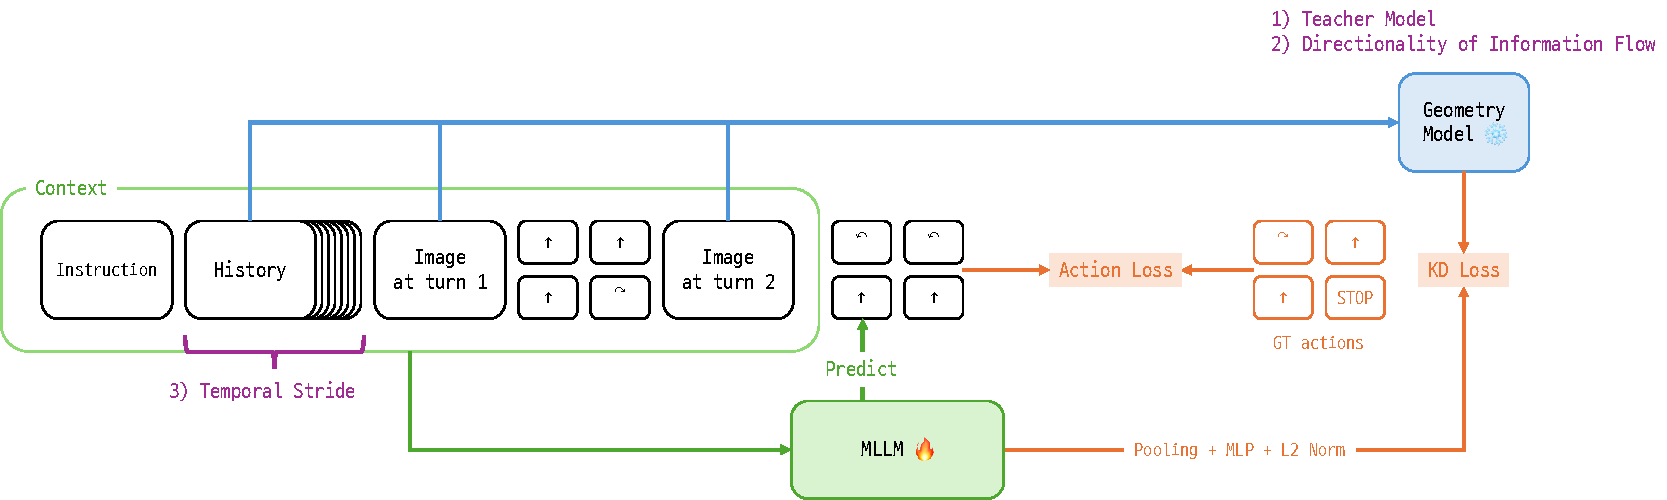
\includegraphics[width=\textwidth]{figs/overall.pdf}
    \caption{Overview of the geometry feature distillation framework for MLLM-based VLN and the three design factors analyzed in this study: (1) teacher model selection, (2) information flow directionality, and (3) temporal stride of navigation history.}
    \label{fig:overall}
\end{figure}
